\documentclass[ignoreframetext]{beamer}
\usepackage[utf8]{inputenc}
\usepackage[T1]{fontenc}
\usepackage[ibycus,swedish,british]{babel}
\usepackage{xparse}
\usepackage{url}
\usepackage{graphicx}
\usepackage{color}
\usepackage{subfig}
\usepackage{multicol}
\usepackage{booktabs}
\usepackage[strict]{csquotes}
\usepackage{cleveref}
\usepackage{amssymb,amsmath,amsthm}

\setbeamertemplate{bibliography item}[text]
\usepackage[natbib,sorting=none,maxbibnames=99]{biblatex}
\addbibresource{bibliography.bib}

\usepackage{bibsp}
\NewFunction{\Enc}{Enc}
\NewFunction{\Dec}{Dec}
\NewFunction{\HMAC}{HMAC}

\usepackage{tikz}
\usetikzlibrary{arrows}


\usetheme{Berlin}
\setbeamertemplate{footline}%{miniframes theme}
{%
  \begin{beamercolorbox}[colsep=1.5pt]{upper separation line foot}
  \end{beamercolorbox}
  \begin{beamercolorbox}[ht=2.5ex,dp=1.125ex,%
    leftskip=.3cm,rightskip=.3cm plus1fil]{author in head/foot}%
    \leavevmode{\usebeamerfont{author in head/foot}\insertshortauthor}%
    \hfill%
    {\usebeamerfont{institute in head/foot}\usebeamercolor[fg]{institute in head/foot}\insertshortinstitute}%
  \end{beamercolorbox}%
  \begin{beamercolorbox}[ht=2.5ex,dp=1.125ex,%
    leftskip=.3cm,rightskip=.3cm plus1fil]{title in head/foot}%
    {\usebeamerfont{title in head/foot}\insertshorttitle} \hfill     \insertframenumber%
  \end{beamercolorbox}%
  \begin{beamercolorbox}[colsep=1.5pt]{lower separation line foot}
  \end{beamercolorbox}
}
\setbeamercovered{transparent}
\setbeamertemplate{bibliography item}[text]

\AtBeginSection[]{%
  \begin{frame}<beamer>
    \tableofcontents[currentsection]
  \end{frame}
}

\ProvideDocumentEnvironment{assumption}{o}{%
  \IfValueTF{#1}{%
    \begin{block}{Assumption: #1}
  }{%
    \begin{block}{Assumption}
  }
}{%
  \end{block}
}

\ProvideDocumentEnvironment{protocol}{o}{%
  \IfValueTF{#1}{%
    \begin{block}{Protocol: #1}
  }{%
    \begin{block}{Protocol}
  }
}{%
  \end{block}
}

\ProvideDocumentEnvironment{remark}{o}{%
  \IfValueTF{#1}{%
    \begin{alertblock}{Note: #1}
  }{%
    \begin{alertblock}{Note}
  }
}{%
  \end{alertblock}
}

\ProvideDocumentEnvironment{idea}{o}{%
  \IfValueTF{#1}{%
    \begin{block}{Idea: #1}
  }{%
    \begin{block}{Idea}
  }
}{%
  \end{block}
}

\ProvideDocumentEnvironment{question}{o}{%
  \setbeamercolor{block body}{bg=orange!15,fg=black}
  \setbeamercolor{block title}{bg=orange,fg=white}
  \setbeamercolor{local structure}{fg=orange}
  \IfValueTF{#1}{%
    \begin{block}{Question: #1}
  }{%
    \begin{block}{Question}
  }
}{%
  \end{block}
}

\ProvideDocumentEnvironment{exercise}{o}{%
  \setbeamercolor{block body}{bg=yellow!10,fg=black}
  \setbeamercolor{block title}{bg=yellow,fg=black}
  \setbeamercolor{local structure}{fg=yellow}
  \IfValueTF{#1}{%
    \begin{block}{Exercise: #1}
  }{%
    \begin{block}{Exercise}
  }
}{%
  \end{block}
}


\begin{document}
\title{%
  Applied Hash Functions
}
\author{Daniel Bosk}
\institute{%
  KTH EECS
}

\begin{frame}
  \maketitle
\end{frame}

\mode<all>
\title{%
  Side-channel attacks
}
\author{Daniel Bosk}
\institute[MIUN ICS]{%
  Department of Information and Communication Systems (ICS),\\
  Mid Sweden University, Sundsvall.
}
\date{\today}


\begin{frame}
  \maketitle{}
\end{frame}


% Since this a solution template for a generic talk, very little can
% be said about how it should be structured. However, the talk length
% of between 15min and 45min and the theme suggest that you stick to
% the following rules:  

% - Exactly two or three sections (other than the summary).
% - At *most* three subsections per section.
% - Talk about 30s to 2min per frame. So there should be between about
%   15 and 30 frames, all told.


\section{Introduction}

\subsection{What are side-channels?}

\begin{frame}
  \begin{definition}[Side Channel]
    A \emph{side channel} is an unintended channel emitting information which 
    is due to physical implementation flaws and not theoretical weaknesses or 
    forcing attempts.
  \end{definition}
  \begin{example}
    Using the standard algorithms for addition and multiplication (using the 
    binary number system) we can easily see that the time to perform \(3\times 
    25\) and \(7\times 25\) will be different.
  \end{example}
\end{frame}

\begin{frame}
  \begin{itemize}
    \item Looking at the numbers we have we see that \(3_{10} = 11_2\), 
      \(7_{10} = 111_2\) and \(25_{10} = 11001_2\)

    \item Assume each step in the algorithm takes one time unit.

    \item Then for \(11001\times 11\) we get:
      \begin{itemize}
        \item \(5\) time units for multiplying the last \(1\) in \(11\) with 
          each digit in \(11001\),

        \item another \(5\) time units for the next digit in \(11\),

        \item we have an additional \(1\) time unit for shifting the second 
          result one step,

        \item finally, we get \(6\) time units for adding the numbers.
      \end{itemize}

    \item For \(11001\times 111\) we get:
      \begin{itemize}
        \item \(5\) time units for each digit, hence \(15\) in total,

        \item we have two shifts, thus \(2\) time units more,

        \item finally we have \(7\) time units for adding.
      \end{itemize}
  \end{itemize}
\end{frame}

\begin{frame}
  \begin{itemize}
    \item Hence, the first multiplication takes \(17\) time units to perform 
      whereas the second takes \(24\) time units.

    \item This is called a timing attack and is one example of why 
      constant-time operations are desirable.

    \item However, in this example we cannot see the difference between 
      multiplication of \(2_{10} = 10_2\) and \(3_{10} = 11_2\).

    \item But in more complex situations this might not even be necessary.

  \end{itemize}
\end{frame}

\subsection{Timing Attacks}

\begin{frame}
  \begin{itemize}
    \item The first example was a timing attack.
    \item We can measure the time for different operations.
    \item Depending on the times it takes we can figure out something about the 
      operands.
  \end{itemize}
\end{frame}

\begin{frame}
  \begin{example}[SSH password guessing]
    \begin{itemize}
      \item In~\cite{song2001timing} a timing attack on passwords sent over 
        encrypted SSH sessions was shown.

      \item As each keystroke in the password is sent in a separate package, 
        the attacker can observe the delay between keystrokes.

      \item They found that this gave a factor 50 advantage for guessing the 
        password.
    \end{itemize}
  \end{example}
\end{frame}

\begin{frame}
  \begin{block}{Anonymized traffic with onion routing}
    \begin{itemize}
      \item Alice sends a message encrypted in three layers to Bob.
      \item Bob removes the outermost layer and sends to Carol.
      \item Carol removes the (next) outermost layer and sends to David.
      \item David removes the final layer and sends to destination.
    \end{itemize}
  \end{block}

  \pause{}

  \begin{example}[De-anonymize traffic]
    \begin{itemize}
      \item We can also perform time-correlation attacks against anonymity 
        systems.

      \item Measure how long it takes between something goes in and something 
        comes out.

      \item Then we can figure out who is sending where.
    \end{itemize}
  \end{example}
\end{frame}

\subsection{Traffic Analysis}

\begin{frame}
\end{frame}

\subsection{Acoustic Attacks}

\begin{frame}
  \begin{itemize}
    \item Some authors\footfullcite{genkin2013rsa} showed an attack to extract 
      a 4096-bit RSA private key from a laptop PC (GnuPG implementation of 
      RSA).

    \item Computers emit high-pitched noise during operation due to some of 
      their electronic components.

    \item This was used to derive the key used for decryption of some chosen 
      ciphertexts within an hour!

    \item Their results show that this attack can be accomplished by placing 
      a mobile phone (microphone) next to the target laptop.
  \end{itemize}
\end{frame}

\begin{frame}
  \begin{figure}
    \includegraphics[height=0.4\textheight]{acoustic-setup.jpg}
  \end{figure}
  \begin{figure}
    \includegraphics[height=0.4\textheight]{acoustic-mobile.jpg}
  \end{figure}
\end{frame}

\begin{frame}
  \begin{figure}
    \includegraphics[height=0.45\textheight]{acoustic-spectrum.jpg}
  \end{figure}
  \begin{itemize}
    \item The acoustic signals are picked up from components in the power 
      supply.

    \item Individual CPU operations are too fast for a microphone to pick up.

    \item But long operations such as modular exponentiation (as in RSA) can 
      create a characteristic acoustic spectral signature which can be detected 
      using a microphone.
  \end{itemize}
\end{frame}

\begin{frame}
  \begin{figure}
    \includegraphics[width=\textwidth]{acoustic-bits.jpg}
  \end{figure}
\end{frame}

\subsection{Physical Attacks}

\begin{frame}
  \begin{figure}
    \includegraphics[width=\textwidth]{physical-setup.png}
  \end{figure}
\end{frame}

\begin{frame}
  \begin{figure}
    \includegraphics[width=\textwidth]{physical-ethernet.png}
  \end{figure}
\end{frame}

\begin{frame}
  \begin{figure}
    \includegraphics[width=\textwidth]{physical-human.png}
  \end{figure}
\end{frame}

\begin{frame}
  \begin{figure}
    \includegraphics[height=0.9\textheight]{physical-spectrum.png}
  \end{figure}
\end{frame}

\subsection{Electromagnetic Attacks}

\begin{frame}
  \begin{figure}
    \includegraphics[height=\textheight]{em-spectrum.png}
  \end{figure}
\end{frame}

\begin{frame}
  \begin{figure}
    \includegraphics[width=\textwidth]{em-pita.png}
  \end{figure}
\end{frame}

\begin{frame}
  \begin{figure}
    \includegraphics[width=\textwidth]{em-pita-detailed.png}
  \end{figure}
\end{frame}

\begin{frame}
  \begin{figure}
    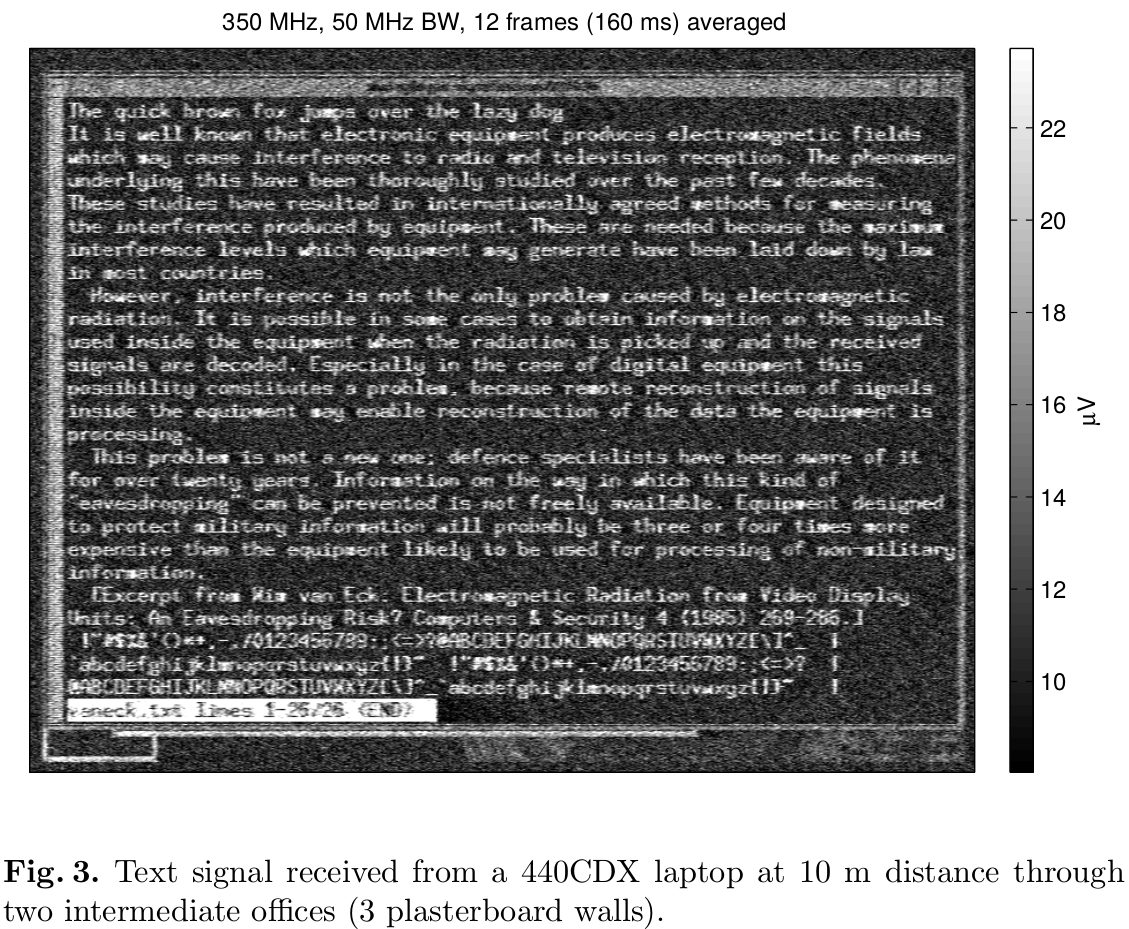
\includegraphics[height=0.9\textheight]{em-laptop.png}
  \end{figure}
  \cite{FlatPanelEmissions}
\end{frame}



%%%%%%%%%%%%%%%%%%%%%%

\begin{frame}{Referenser}
  \small
  \printbibliography{}
\end{frame}


\mode*

\begin{frame}[allowframebreaks]
  \printbibliography
\end{frame}
\end{document}
